\documentclass[11pt]{article}

\usepackage[letterpaper]{geometry}

\usepackage[utf8]{inputenc}
\usepackage{mathpazo}
\usepackage{amsmath}
\usepackage{amsfonts}
\usepackage{physics}
\usepackage{siunitx}

\usepackage{fancyhdr}

\usepackage{graphicx}
\usepackage{float}
\usepackage{booktabs}

\usepackage[shortlabels,inline]{enumitem}

% Hyperlinks with decent looking default colors.
\usepackage{hyperref}
\usepackage{xcolor}
\hypersetup{
  colorlinks,
  linkcolor={red!50!black},
  citecolor={blue!50!black},
  urlcolor={blue!80!black}
}

% For those sexy spaced low small caps from classic-thesis!
\usepackage{microtype}
\usepackage{textcase}
\DeclareRobustCommand{\spacedlowsmallcaps}[1]{%
  \textls[80]{\scshape\MakeTextLowercase{#1}}%
}

% Replaced mathpazo \sum symbol with computer modern's.
\DeclareSymbolFont{cmlargesymbols}{OMX}{cmex}{m}{n}
\let\sumop\relax
\DeclareMathSymbol{\sumop}{\mathop}{cmlargesymbols}{"50}

\newcommand{\forceindent}{\leavevmode{\parindent=1em\indent}}

\pagestyle{fancy} 
\fancyhead{}
\rhead{Ali Ramadhan}
\chead{}
\lhead{12.818: Project 4}
\cfoot{}
\rfoot{\thepage}

\title{\spacedlowsmallcaps{\small 12.818: Introduction to Atmospheric Data and Large-scale Dynamics}\\ \spacedlowsmallcaps{\Large Project four: The meridional structure of the atmosphere}}
\author{\spacedlowsmallcaps{Ali Ramadhan}}
\date{}

% \renewcommand\thesection{\Alph{section}}

\begin{document}
\maketitle

In this project we will investigate the nature of convection in the lower troposphere, which is the mechanism responsible for transporting heat from terrestrial radiation vertically upward to the upper troposphere where water vapor concentration and thus infrared absorption is much lower, allowing it to be emitted to outer space.

\begin{figure}[h!]
  \centering
  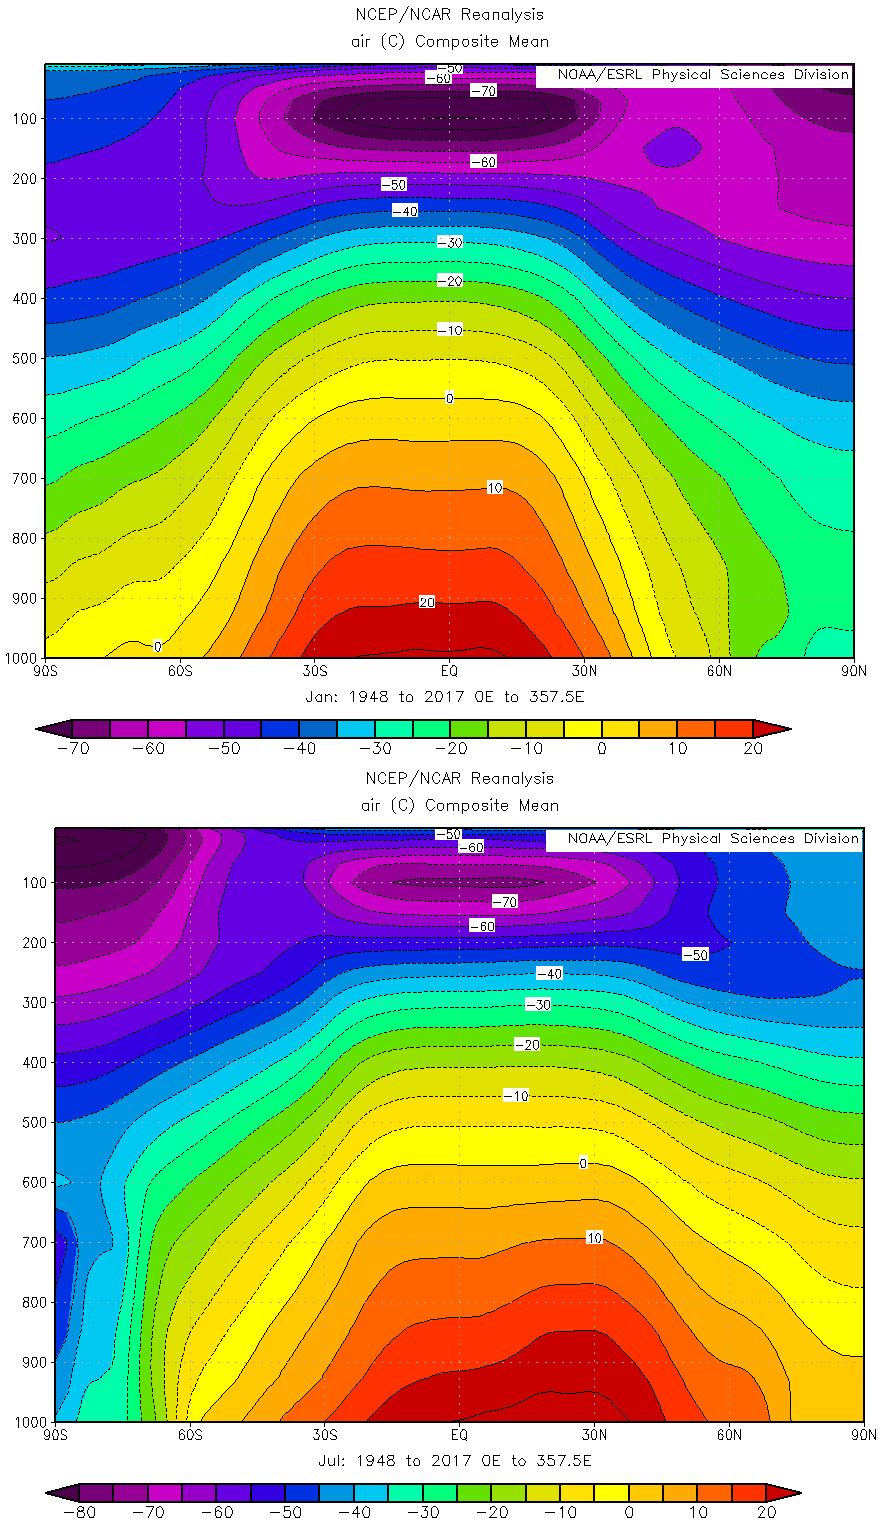
\includegraphics[width=0.8\textwidth]{airT_janjul.png}
  \caption{Zonally averaged surface air temperatures (in \SI{}{\degreeCelsius}) for the months of January and July produced using using NCEP reanalysis data averaged over the years 1948--2017.}
  \label{fig:airT}
\end{figure}

\begin{figure}[h!]
  \centering
  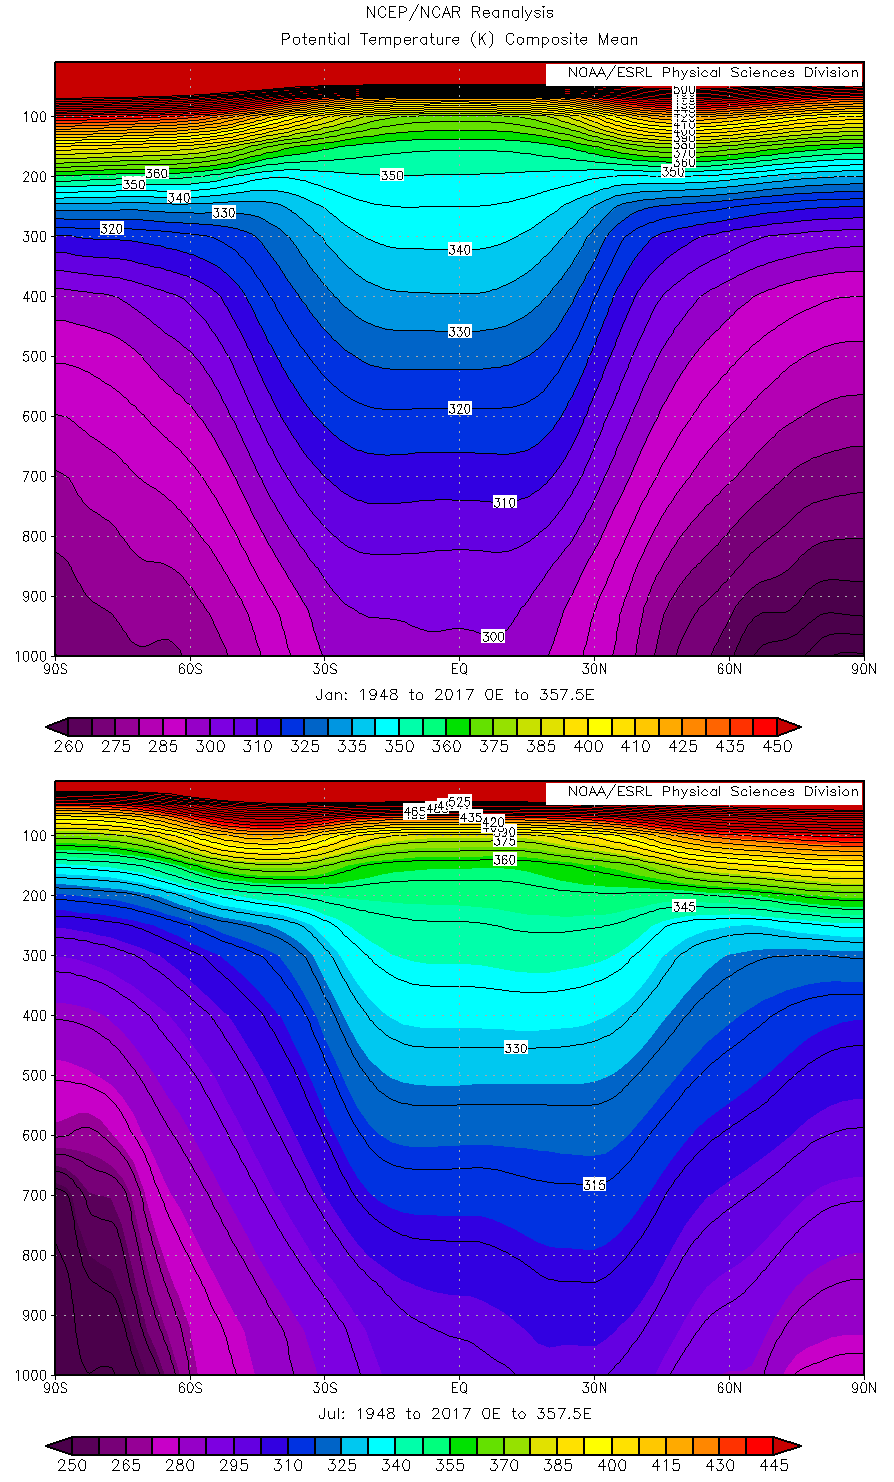
\includegraphics[width=0.8\textwidth]{theta_janjul.png}
  \caption{Zonally averaged potential temperatures (in units of Kelvin) for the months of January and July produced using using NCEP reanalysis data averaged over the years 1948--2017.}
  \label{fig:theta}
\end{figure}

\begin{figure}[h!]
  \centering
  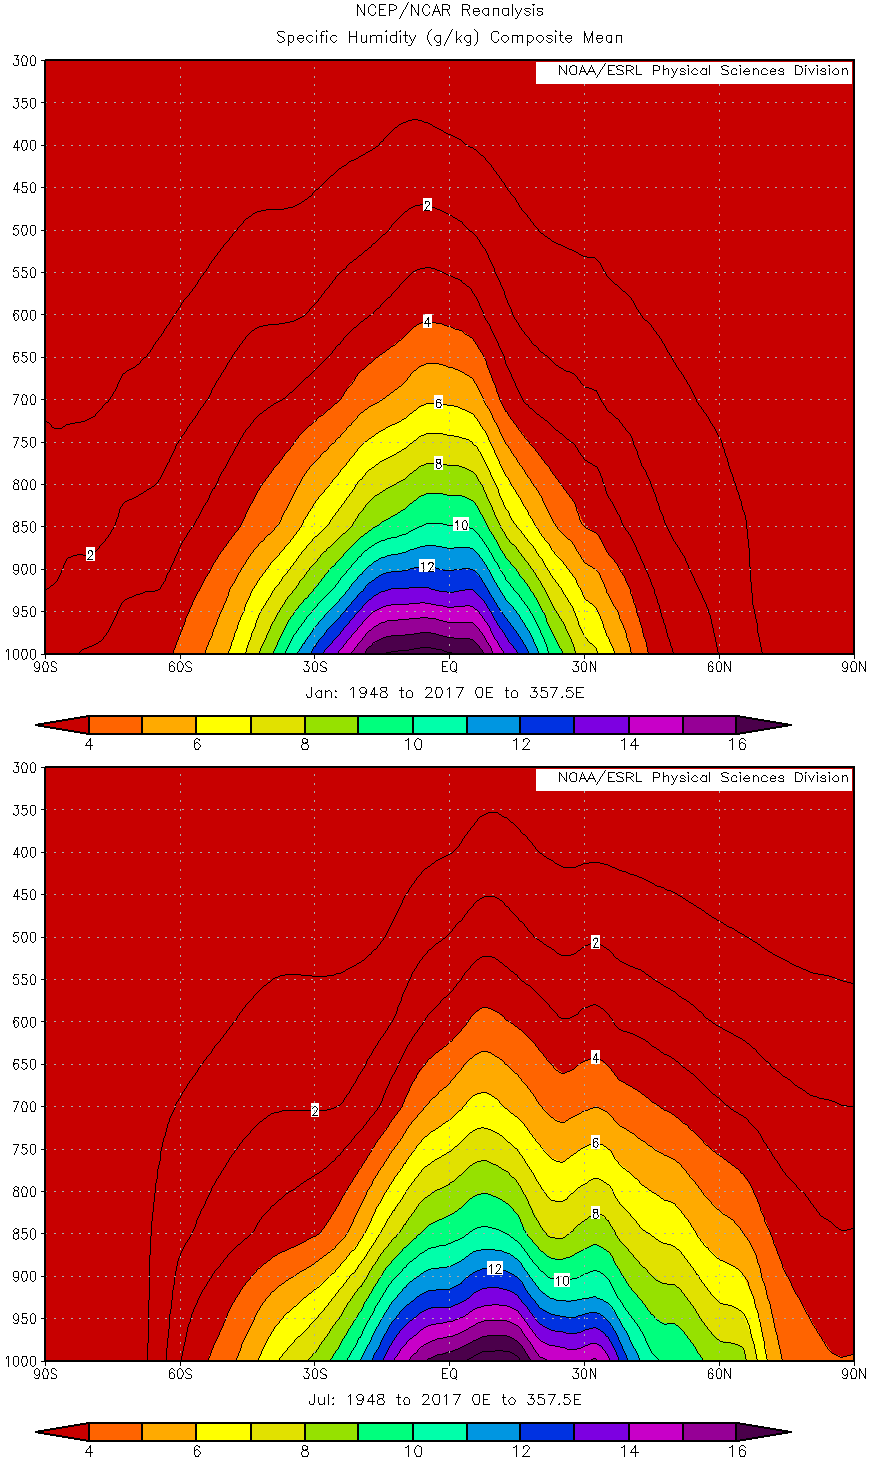
\includegraphics[width=0.8\textwidth]{qstar_janjul.png}
  \caption{Zonally averaged specific humidity (in \SI{}{\g/\kg}) for the months of January and July produced using using NCEP reanalysis data averaged over the years 1948--2017.}
  \label{fig:qstar}
\end{figure}

\begin{figure}[h!]
  \centering
  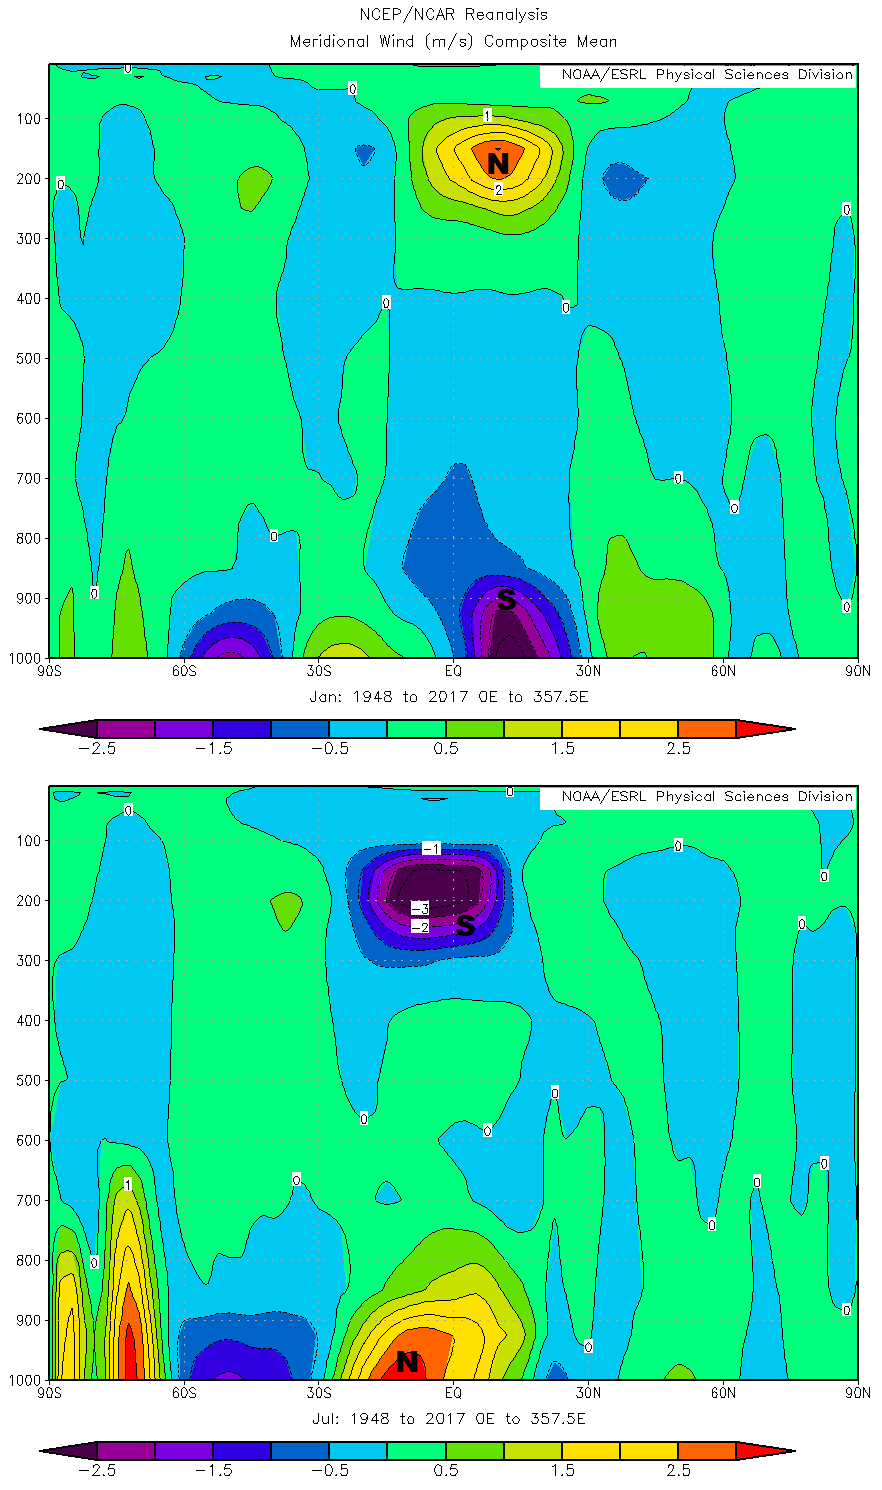
\includegraphics[width=0.8\textwidth]{mer_wind_janjul.png}
  \caption{Zonally averaged meridional wind (in \SI{}{\m/\s}) for the months of January and July produced using using NCEP reanalysis data averaged over the years 1948--2017.}
  \label{fig:mer_wind}
\end{figure}

\begin{figure}[h!]
  \centering
  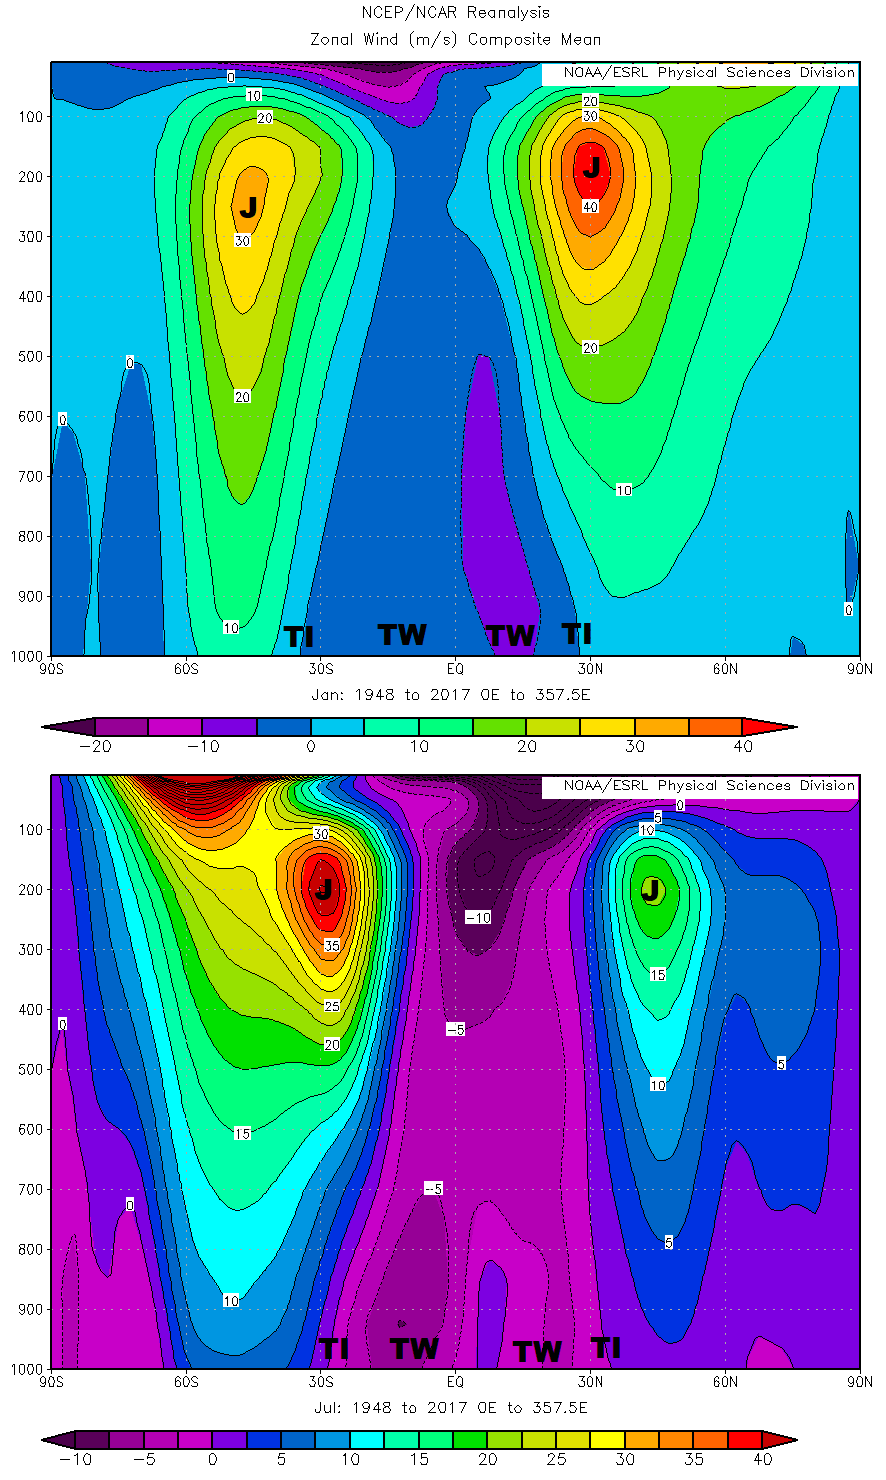
\includegraphics[width=0.8\textwidth]{zonal_wind_janjul.png}
  \caption{Zonally averaged zonal wind (in \SI{}{\m/\s}) for the months of January and July produced using using NCEP reanalysis data averaged over the years 1948--2017.}
  \label{fig:zonal_wind}
\end{figure}

\begin{figure}[h!]
  \centering
  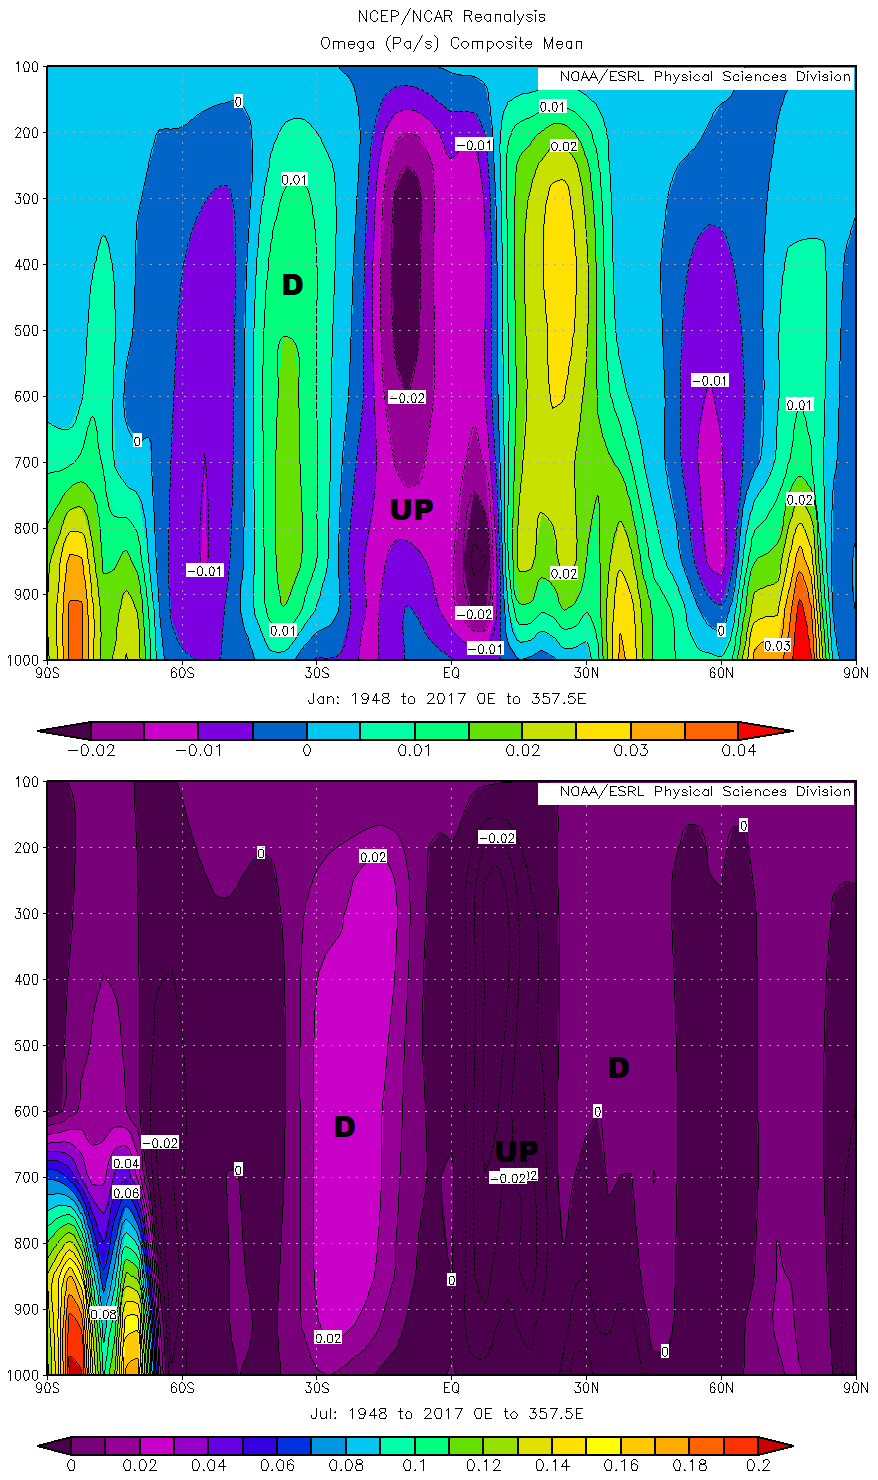
\includegraphics[width=0.8\textwidth]{omega_janjul.png}
  \caption{Zonally averaged vertical velocities (in \SI{}{\Pa/\s}) for the months of January and July produced using using NCEP reanalysis data averaged over the years 1948--2017.}
  \label{fig:omega}
\end{figure}


%\begin{thebibliography}{9}
%\bibitem{AMSVirtualTemp}
%American Meteorological Society, cited 2012: Virtual temperature. Glossary of Meteorology. [Available online at \url{http://glossary.ametsoc.org/wiki/Virtual_temperature}]
%
%\bibitem{Wallace}
%Wallace, John M. and Peter V. Hobbs. \textit{Atmospheric Science; An Introductory Survey}. Elsevier. Second Edition, 2006. Chapter 1.
%\end{thebibliography}

\end{document}